\newpage
\subsection{Widerstandsmessung IV: Impedanzen}\label{sec:1-4}

\begin{highlightblock}[Messung Impedanzen, Drei-Voltmeter-Methode]
    Funktionsgenerator $20\mathrm{V_{SS}}$. $50\Omega$ Shuntwiderstand, 
    \begin{enumerate}[label=\textbf{\alph*:}, ref=\alph*]
        \item\label{itm:1-P4-1} Frequenz geeignet wählen.
        \item\label{itm:1-P4-2} Spannungsdreieck zeichnen. Daraus Betrag und Phase ablesen.
        \item\label{itm:1-P4-3} Ergebnis mit der Rechnung vergleichen.
    \end{enumerate}
\end{highlightblock}

\subsubsection{Verwendetes Material}

\begin{table}[h]
	\centering
	\caption{Verwendetes Material}
	\begin{tabularx}{\textwidth}{XXX}
		\textbf{Messgerät} & \textbf{Verwendung} & \textbf{Anmerkungen}\\ \midrule
		&  &  \\
		&  &  \\
		&  &  \\
	\end{tabularx}	
\end{table}

\subsubsection{Versuchsaufbau}

\marginref{\ref{itm:1-P4-1}}
Für die Frequenz wurde $f=\SI{1}{\kilo\hertz}$ gewählt. Bei dem
Frequenzgenerator war es nur möglich $\SI{10}{\volt}_{PP}$ einzustellen.
Anstelle von $R$ wurde ein Shuntwiderstand von $R=\SI{50}{\ohm}$ verwendet.
$Z$ ist hier entweder die zur verfügung gestellte Spule oder der Kondensator.

\begin{figure}[h]
    \centering
    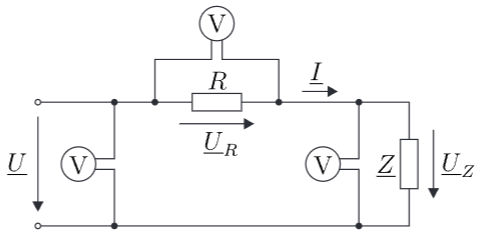
\includegraphics[width=7cm]{images/14_Aufbau.png}
    \caption{Aufbau der Messung}\label{fig:14-aufbau}
\end{figure}

\marginref{\ref{itm:1-P4-2}}

Für die drei Messgeräte ergeben sich folgende Einzelmesswerte:

\begin{table}[h]
    \caption{Messergebnisse der 3-Voltmeter-Methode}\label{tab:14-values}
    \begin{tabularx}{\textwidth}{XYYY}
        \textbf{Bauteil} & $U / \si{\volt}$ & $U_R / \si{\volt}$ & $U_Z / \si{\volt}$ \\ \midrule
        Kondensator & 3.45 & 3.367 & 0.315 \\
        Spule & 5.534 & 2,151 & 4.807
    \end{tabularx}
\end{table}

\newpage

Mit diesen Effektivwerten der Spannungen können nun die Spannungsdreiecke
mit Lineal und Zirkel konstruiert werden, oder wie hier in GeoGebra:

\begin{figure}[h]
\begin{minipage}[position]{0.48\textwidth}
    \centering
    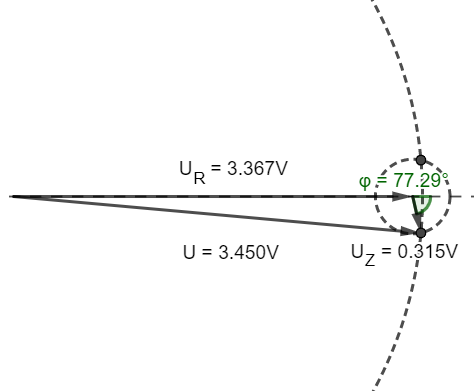
\includegraphics[height=4.5cm]{images/14_3-Voltmeter_C.png}
    \caption{Spannungsdreieck des Kondensators}
\end{minipage}\hfill
\begin{minipage}[position]{0.48\textwidth}
    \centering
    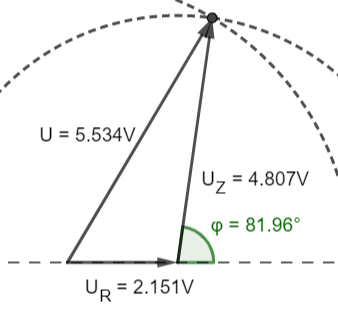
\includegraphics[height=4.5cm]{images/14_3-Voltmeter_L.png}
    \caption{Spannungsdreieck der Spule}
\end{minipage}
\end{figure}

Formeln für Betrag und Phase der Impedanz~\cite[S.~21]{EMTPraktikum2025}:

\[
    |Z| = \frac{U_C}{U_R/R} \qquad |\varphi_C| = \arccos\left(\frac{U^2-U_R^2-U_Z^2}{2U_Z U_R}\right)
\]

\begin{minipage}[t]{0.48\textwidth}

    Da bekannt ist, dass die gemessene impedanz Kapazitiv ist, ist das Vorzeichen des Winkels negativ.

    \[
        \begin{aligned}
            |Z_C| &= \frac{\SI{0.315}{\volt}}{\SI{3.367}{\volt}/\SI{50}{\ohm}} = \SI{4.678}{\ohm} \\
            \varphi_C & = \SI{-1.349}{\radian} = \SI{-77.3}{\degree}\\
        \end{aligned}
    \]

\end{minipage}\hfill
\begin{minipage}[t]{0.48\textwidth}

    Da bekannt ist, dass die gemessene impedanz Induktiv ist, ist das Vorzeichen des Winkels positiv.

    \[
        \begin{aligned}
            |Z_L| &= \frac{\SI{4.807}{\volt}}{\SI{2.151}{\volt}/\SI{50}{\ohm}} = \SI{111.7}{\ohm} \\
            \varphi_L &= \SI{1.431}{\radian} = \SI{82.0}{\degree} \\
        \end{aligned}
    \]

\end{minipage}

\marginref{\ref{itm:1-P4-3}}
Um die einzelnen Werte der Komponenten zu erhalten, werden die Impedanzen in in
Real- und Imaginärteil zerlegt: $Z = R + \jmath X$

\begin{minipage}[position]{0.48\textwidth}
    \[
        \begin{aligned}
            R_C &= |Z_C| \cdot \cos(\varphi_C) = \SI{1.029}{\ohm} \\
            \jmath X_C &= \jmath |Z_C| \cdot \sin(\varphi_C) = -\jmath\SI{4.536}{\ohm}
        \end{aligned}
    \]
\end{minipage}\hfill
\begin{minipage}[position]{0.48\textwidth}
    \[
        \begin{aligned}
            R_L &= |Z_L| \cdot \cos(\varphi_L) = \SI{15.62}{\ohm} \\
            \jmath X_L &= \jmath |Z_L| \cdot \sin(\varphi_L) = \jmath\SI{111.7}{\ohm}
        \end{aligned}
    \]
\end{minipage}

\medskip
Umrechnen in Kapazität und Induktivität und den äquivalenten Serienwiderstand (ESR), jeweils bei $f=\SI{1}{\kilo\hertz}$:

\begin{minipage}[position]{0.48\textwidth}
    \[
        \begin{aligned}
            C &= -\frac{1}{2\pi f X_C} = \SI{35.1}{\micro\farad} \\
            R_{\mathrm{ESR}} &= R_C = \SI{1.029}{\ohm}
        \end{aligned}
    \]
\end{minipage}\hfill
\begin{minipage}[position]{0.48\textwidth}
    \[
        \begin{aligned}
            L &= \frac{X_L}{2\pi f} = \SI{17.8}{\milli\henry} \\
            R_{\mathrm{ESR}} &= R_L = \SI{15.62}{\ohm}
        \end{aligned}
    \]
\end{minipage}

\subsubsection{Erkenntnisse}

Hier wurde unglücklicherweise der Vorwiderstand von $R_V=\SI{68}{\ohm}$ bei der
Kondensatormessung nicht berücksichtigt, was zu einem schlechtem Verhältnis von
$U_Z$ zu $U_R$ führt. Dadurch wirken sich Messfehler bei den gemessenen
Spannungen stärker auf das Ergebnis aus. Weiters hätte die Frequenz beider
Messungen angepasst werden können, sodass bei den Impedanzen und dem
Shunt-Widerstand etwa die selbe Spannung abfällt, um den Messbereich weiter zu
verbessern.

% Beispielrechnung einfügen